\documentclass{article}
\usepackage[final]{neurips}
\usepackage[framemethod=tikz]{mdframed}
\usepackage{lipsum}
\definecolor{mycolor}{rgb}{0.122, 0.435, 0.698}
\newmdenv[innerlinewidth=0.5pt, roundcorner=4pt,linecolor=mycolor,innerleftmargin=6pt,
innerrightmargin=6pt,innertopmargin=6pt,innerbottommargin=6pt]{mybox}
\usepackage[utf8]{inputenc} % allow utf-8 input
\usepackage[T1]{fontenc}    % use 8-bit T1 fonts
\usepackage[hidelinks]{hyperref}       % hyperlinks
\usepackage{url}            % simple URL typesetting
\usepackage{booktabs}       % professional-quality tables
\usepackage{amsfonts}       % blackboard math symbols
\usepackage{nicefrac,tcolorbox}       % compact symbols for 1/2, etc.
\usepackage{amsmath}
\usepackage{enumitem}
\usepackage{microtype}      % microtypography
\usepackage{graphicx,caption}
\usepackage{xepersian}
\settextfont{XB Niloofar}
\setdigitfont{XB Niloofar}
\raggedbottom


\title{
	\vspace{-0.8em}
سوالات اضافی عید - درس نظریه گروه‌ها - دکتر رضاخانی
\\
{\normalsize
\textbf{
برای تمرین بیشتر و تسلط روی مفاهیم
\\
\vspace{-0.4em}
تحویل (اجباری نیست)
از طریق سامانه
\href{https://cw.sharif.edu/}{درس‌افزار شریف}
}
}
\vspace{-0.6em}
}

\usepackage[utf8]{inputenc}

\usepackage[english]{babel}
\setlength{\parindent}{3.5em}
\setlength{\parskip}{0.5em}
\renewcommand{\baselinestretch}{1.0}

\usepackage{calrsfs}
\DeclareMathAlphabet{\pazocal}{OMS}{zplm}{m}{n}
\newcommand{\La}{\mathcal{L}}
\newcommand{\Lb}{\pazocal{L}}

\newtcolorbox{boxes}[3][]
{
	colframe = #2!25,
	colback  = #2!10,
	coltitle = #2!40!black,  
	title    = {\textbf{#3}},
	#1,
}

\newenvironment{exercise}[3][\unskip]{%
	\par
	\noindent
	\textbf{تمرین
		#1
		[#2 امتیاز] 
		\def\temp{#3}\ifx\temp\empty
		: 
		\else
		: #3 \vspace{0.5em} \\ \noindent
		\fi
}}{}

\author{
حسین محمدی\\
  \lr{
  		\href{mailto:hossein.mohammadi.00427@gmail.com}{\texttt{	hossein.mohammadi.00427@gmail.com}}} \\
  \And
  زهرا کبیری\\
 \lr{
  		\href{mailto:kabiri.zahra98@gmail.com}{ \texttt{kabiri.zahra98@gmail.com}}}\\
  }

\begin{document}


\begin{minipage}{0.1\textwidth}% adapt widths of minipages to your needs
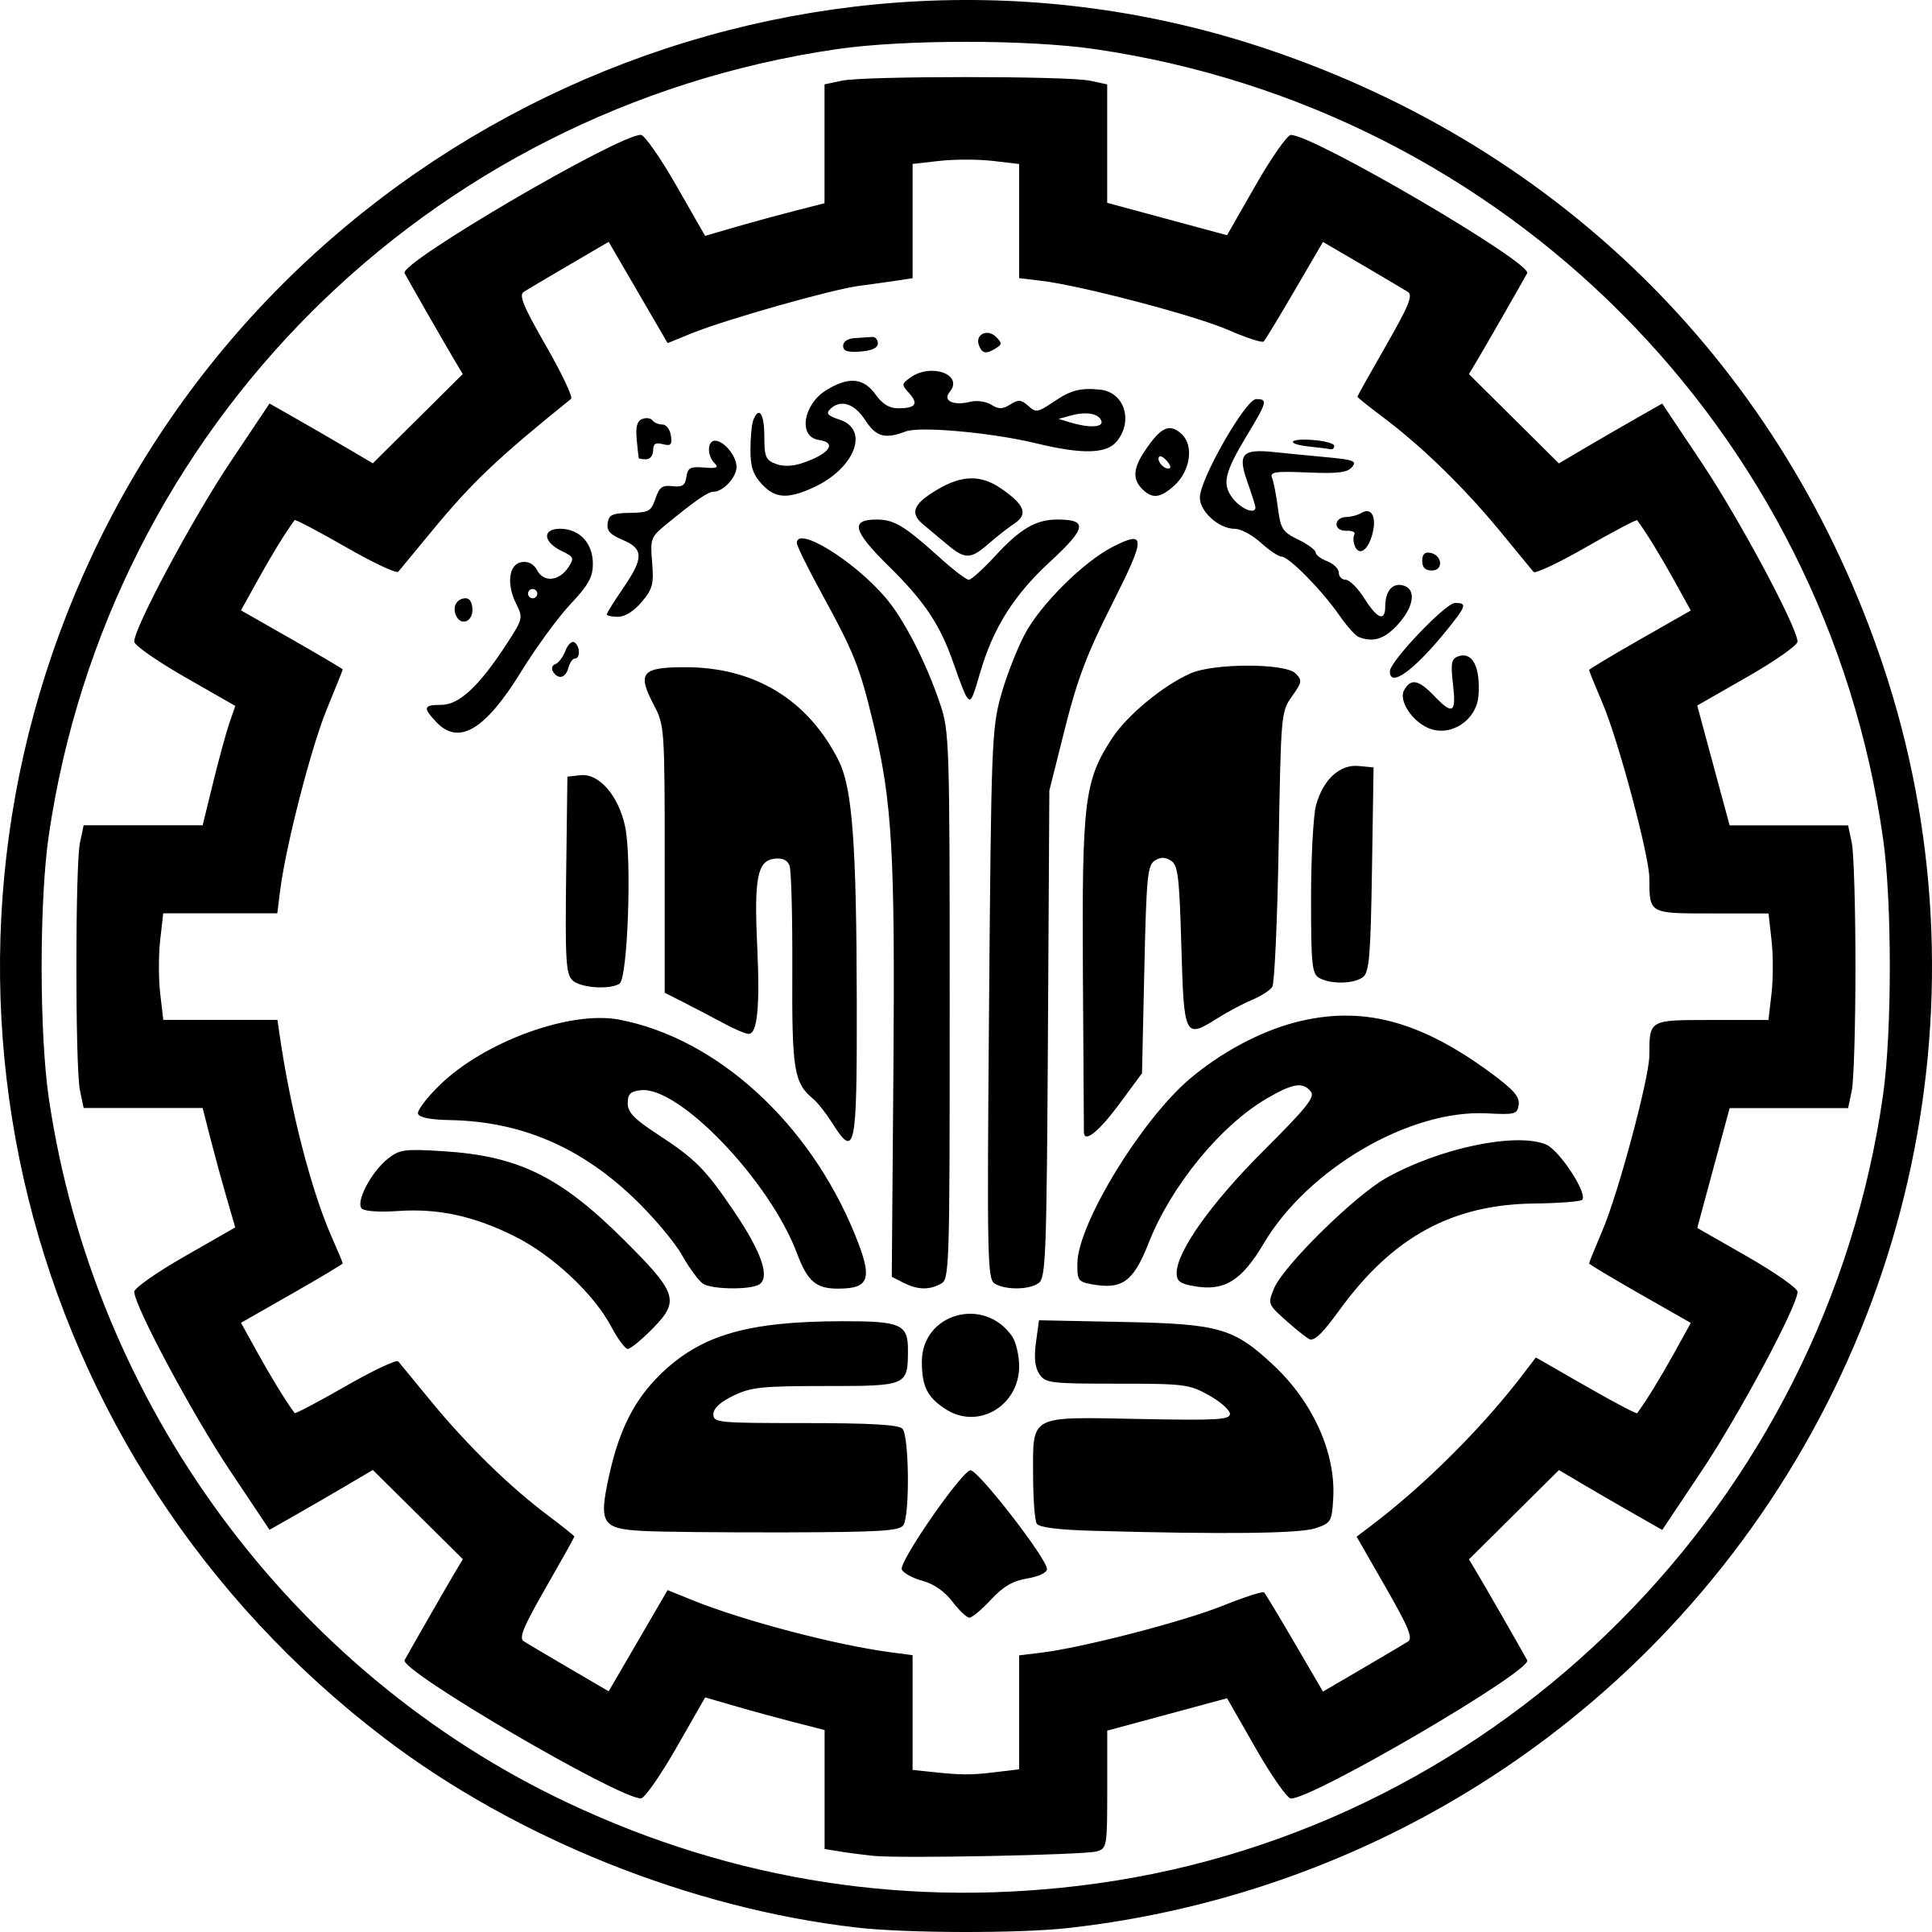
\includegraphics[width=1.1cm]{sharif-logo.png}
\end{minipage}%
\hfill%
\begin{minipage}{0.9\textwidth}\raggedleft
دانشگاه صنعتی شریف\\
زمستان ۱۴۰۲ - بهار ۱۴۰۳\\
\end{minipage}

\makepertitle


\begin{exercise}[
	$1^\prime$
	]{-}{}
	فرض کنید $H$ و $K$ دو زیرگروه از یک گروه $G$‌ باشند. 
	
	\noindent
	الف) نشان دهید که 
	$H\cup K$
	\textbf{فقط و فقط}
	وقتی یک زیرگروه از 
	$G$ 
	است که یکی از 
	$H$
	یا
	$K$
	مشمول در دیگری باشد.
	
	\noindent
	ب) نتیجه بگیرید که هیچ گروهی اجتماع دو زیرگروه سره خود نیست.
	
\end{exercise}
\vspace{1em}

\begin{exercise}[
	$2^\prime$
	]{-}{}
	نشان دهید تعداد زیرگروه‌های یک گروه نامتناهی، نامتناهی است.
	
\end{exercise}
\vspace{1em}

\begin{exercise}[
	$3^\prime$
	]{-}{}
 گروه	$G$ 
	 را یک گروه متناهی درنظر بگیرید که  
	$A$ و 
	$B$
	دو زیرمجموعه‌ی ناتهی از آن هستند به گونه‌ای که 
	$|A|+|B| > |G|$.
	 نشان دهید
	 	 \LTRfootnote{$AB = \{ab \big| a\in A , b\in B\}$}
	  $AB = G$.
	  همچنین
 با مثالی نشان دهید که اگر 
 $|A|+|B| = |G|$
 این نتیجه‌گیری ممکن است نادرست باشد.
\end{exercise}
\vspace{1em}

\begin{exercise}[
	$4^\prime$
	]{-}{}
	فرض کنید 
	$a$و $b$
	دو عنصر از مرتبه‌ی متناهی در گروه 
	$G$ باشند که
	$ab=ba$.
	صحت یا سقم احکام زیر را بررسی کنید.
	
	\noindent
	\vspace{0.25em}
	الف) اگر 
	$\left< a\right>\cup \left< b\right> = {e}$
	آنگاه
	\footnote{مقصود از 
	$o(a)$ مرتبه‌ی عضو $a$ از گروه است. همچنین نماد
	$[x,y]$
	ک.م.م. دو عدد صحیح $x$ و $y$‌را نشان می‌دهد.}
	$o(ab) = [o(a),o(b)]$.
	
	\noindent
	\vspace{0.25em}
	ب) اگر $o(ab) = [o(a),o(b)]$ آنگاه $\left< a\right>\cup \left< b\right> = {e}$.
	
	\noindent
	\vspace{0.25em}
	ج) گروه $G$ دارای یک عضو $c$ است به طوری‌که 
	$o(c) = [o(a),o(b)]$.
\end{exercise}
\vspace{1em}

\begin{exercise}[
	$5^\prime$
	]{-}{}
	فرض کنید گروه $G$ یک گروه متناهی باشد که مرتبه‌اش بر 3 بخش‌پذیر نیست و همچنین به ازای هر دو عضو 
	$a$ و $b$ از گروه $G$ داشته باشیم: 
	$(ab)^3 = a^3b^3$.  نشان دهید که گروه 
	$G$ باید آبلی باشد.
\end{exercise}
\vspace{1em}

\begin{exercise}[
	$6^\prime$
	]{-}{}
	فرض کنید گروه 
	$G$ گروه آبلی باشد و اعضای 
	$a$ و $b$ به ترتیب دارای 
	مرتبه‌های 
	$m$ و $n$  باشند. نشان دهید که 
	$G$ عضوی دارد که مرتبه‌اش 
	ک.م.م. $m$ و $n$ است.
\end{exercise}
\vspace{1em}


\begin{exercise}[
	$7^\prime$
	]{-}{}
	فرض کنید گروه $G$ گروه آبلی متناهی‌ای باشد که تعداد حل‌های معادله 
	$x^n =e$
	(برای هر عدد طبیعی $n$)
	در $G$، حداکثر $n$ باشد. نشان دهید که $G$ گروه دوری است. 
\end{exercise}
\vspace{1em}

\begin{exercise}[
	$8^\prime$
	]{-}{}
	اگر $a^5=e$  و  
	$aba^{-1} = b^2$
	باشد، مرتبه‌ی عضو $b$ چه اعدادی می‌تواند باشد؟ (نیاز نیست روی گروه $G$ که اعضای $a$و$b$ از آن اختیار می‌شوند، فرض خاصی کنیم.) 
\end{exercise}
\vspace{1em}

\begin{exercise}[
	$9^\prime$
	]{-}{}
	گروه $G$ به گونه‌ای است که اشتراک تمامی زیرگروه‌های غیربدیهی‌اش، نابدیهی است
	\footnote{منظور از زیرگرو‌ه‌های بدیهی، کل گروه و زیرگروه 
	$\{e\}$
	است.}. نشان دهید که هر عضو از گروه $G$ مرتبه‌ی متناهی دارد.
\end{exercise}
\vspace{1em}

\begin{exercise}[
	$10^\prime$
	]{-}{}
	گروه $G$ را گروه آبلی متناهی از مرتبه‌ی 
	$o(G)$
	در نظر بگیرید. فرض کنید عدد طبیعی $n$ نسبت به مرتبه‌ی گروه اول باشد. نشان دهید که هر عضو 
	$g\in G$ 
	می‌تواند به شکل 
	$g=x^n$
	نوشته شود، برای یک عضو مشخص 
	$x\in G$.
	
\end{exercise}
\vspace{1em}

\begin{exercise}[
	$11^\prime$
	]{-}{}
	نشان دهید که هر گروه از مرتبه‌ی ۹ حتما آبلی است.
\end{exercise}
\vspace{1em}

\begin{exercise}[
	$12^\prime$
	]{-}{}
	مثالی از یک گروه غیرآبلی بزنید که برای تمامی اعضای 
	$a,b\in G$
	داشته باشیم:
	$(ab)^3 = a^3b^3$
\end{exercise}
\vspace{1em}

\begin{exercise}[
	$13^\prime$
	]{-}{کار با جایگشت‌ها و دورها}	
	\noindent
الف) نشان دهید که 
\[
(1,2,3,\dots, n)^{-1} = (n,n-1,\dots,3,2,1)
\]
	\noindent
	\vspace{0.25em} 
	ب) برای چه عدد طبیعی 
	$m$، دورهای به طول 
	$m$ زوج هستند؟
	
	\noindent
	\vspace{0.25em}
	ج) نشان دهید کوچکترین زیرگروهی که شامل دو عضو 
	$(12)$
	و
	$(123\dots n)$
	باشد، خود گروه 
	$S_n$
	است.
\end{exercise}
\vspace{1em}

\begin{exercise}[
	$14^\prime$
	]{-}{}
	نشان دهید مجموعه‌ی تمام جایگشت‌های زوج از گروه $S_n$، خود تشکیل یک گروه می‌دهد؛ این گروه را 
	$A_n$
	می‌نامیم.
\end{exercise}
\vspace{1em}

\begin{exercise}[
	$15^\prime$
	]{-}{}
	نشان دهید گروه 
	$A_n$
	با دورهای به طول سه تولید می‌شود.
\end{exercise}
















 \end{document}
